\chapter{ランサムウェア対策}
\section{感染リスクの緩和}
現実世界の攻撃を戦術と使用技術の観点から分類したフレームワークであるMITRE ATT\&CK \cite{MITREATT12:online}によると,
ランサムウェアのデータ侵害は,攻撃の最終段階であるImpactステージの
Data Destruction,
Data Encrypted for Impact,
Data Manipulation
のいずれかに分類される.
つまり,ランサムウェアによるデータ侵害はInitial Access (初期アクセス) や Privilege Escalation (権限昇格) などのステージを完了した後に発生するといえる.
したがって,Impactより前のステージにおけるセキュリティ強化もランサムウェア対策の重要な要素である.
なお,本研究の提案手法はランサムウェアのImpactステージの活動に対する対策であるため,本節の内容はスコープ外であることに注意する.
\begin{figure}[t]
  \begin{center}
    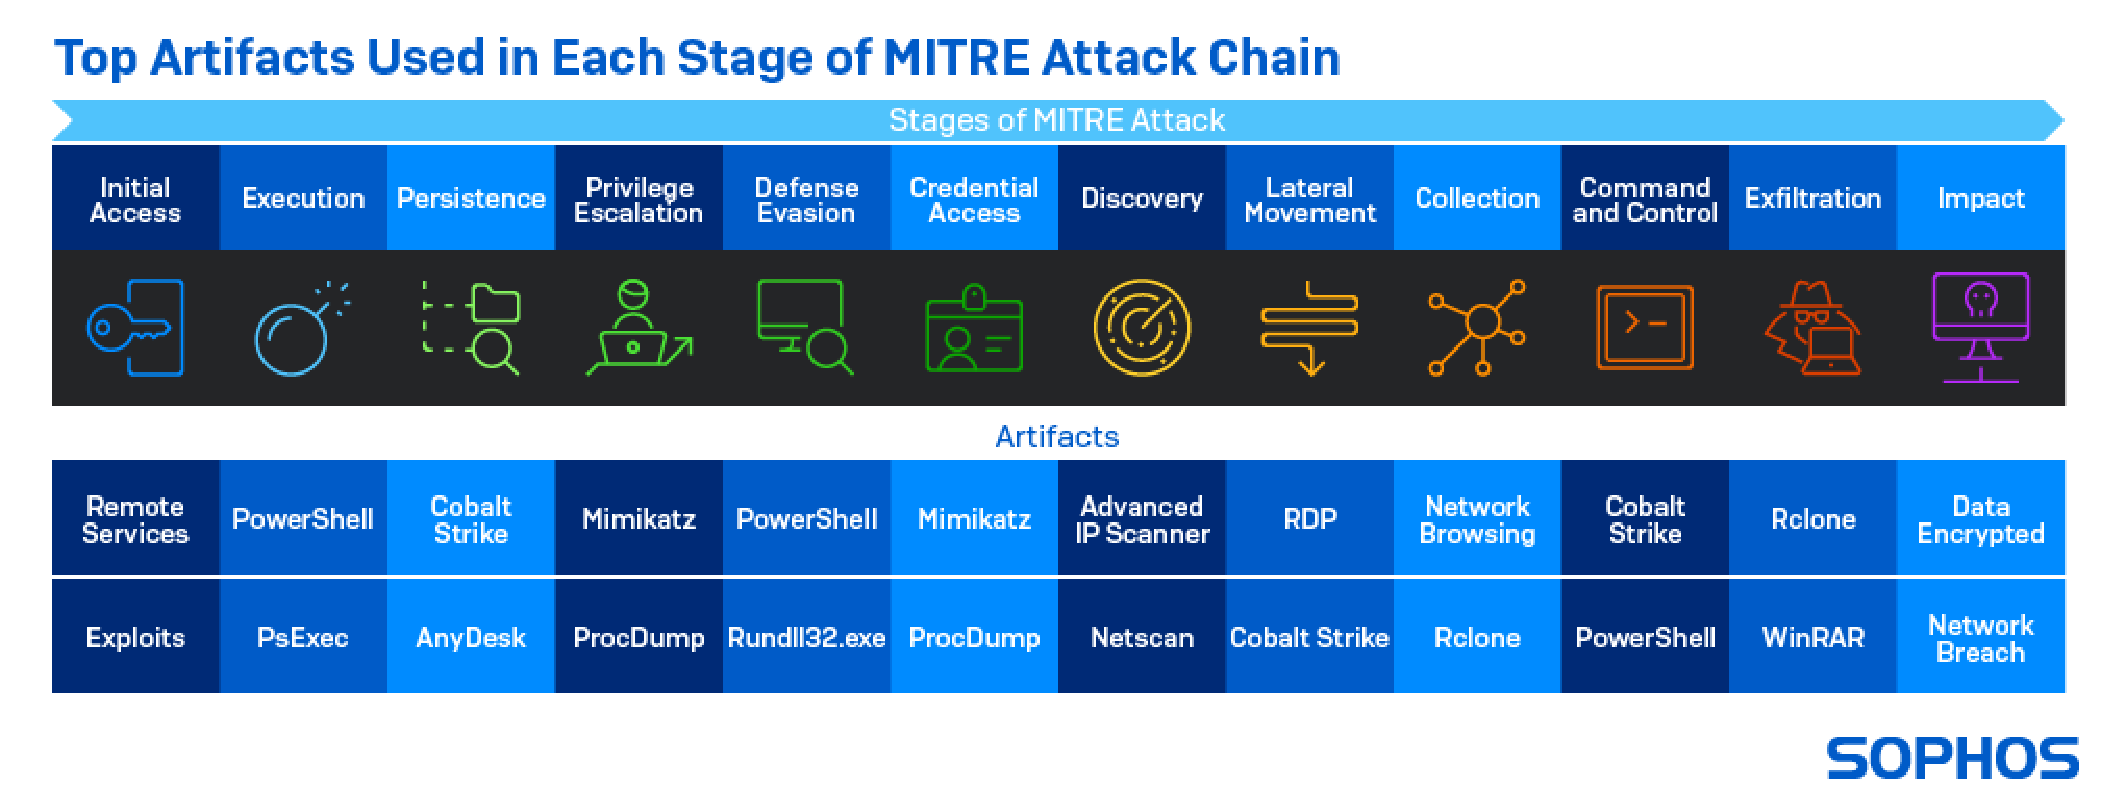
\includegraphics[width=0.8\columnwidth]{doc/img/mitre-attack-chain.eps}
  \end{center}
  \caption{Overview of each stage in MITRE ATT\&CK framework.
    Some stages such as Reconnaissance are omitted for simplicity. \cite{mitre-explained}}
  \label{fig:mitre-attack-chain}
\end{figure}

本節では,すべてのランサムウェアが通過するステージであるInitial Accessステージに焦点を当て,感染リスクの緩和について述べる.
SpyCloud社 \cite{spycloud-ransomware} によると,ランサムウェアのInitial Accessに利用される手法として2023年に最も多く報告されたものは
フィッシング,サードパーティアプリケーションのIAM設定の不備,cookie窃取によるセッションハイジャックであった.
これらの手法に対する一般的な対策を\tabref{tab:initial-access}に示す.
\begin{table}[t]
  \centering
  \label{tab:initial-access}
  \caption{Techniques for Initial Access and general countermeasures}
  \begin{tabular}{|c|c|}
    \hline
    \textbf{Techniques for Initial Access} & \textbf{Countermeasures} \\
    \hline
    Phishing                               &
    \begin{tabular}{c}
      Email filtering \\ User awareness training
    \end{tabular}
    \\
    % Email filteringUser awareness training,         \\
    \hline
    Misconfigured IAM settings             &
    \begin{tabular}{c}
      Multi factor authentication \\ Regular audit
      % Email filtering \\ User awareness training
    \end{tabular}
    \\
    \hline
    Session hijacking through cookie theft &
    \begin{tabular}{c}
      Enable Secure and HTTPOnly attribute \\
      Multi factor authentication
    \end{tabular}
    \\
    \hline
  \end{tabular}
\end{table}

